\chapter{Topics in String Theory}

These notes follow Leonard Susskind's ninth lecture in the supplementary Cosmology and Black Holes track, and are curated as companion notes by LazyingArt LLC. The lecture begins from a student's concrete question, how a cosmic horizon can be hot at all, and builds outward from that question. The route is deliberate: black-hole horizon thermodynamics first, then de Sitter geometry for a single observer, then the Newtonian potential associated with vacuum energy, and finally the statistical mechanics of a finite-entropy causal patch, with recurrences, Boltzmann brains, eternal inflation, and the measure problem appearing as natural extensions of the same line of thought.

\section{Horizons Are Always Hot}

Susskind opens by refusing to treat ``horizons are hot'' as a slogan. The statement is operational. If one lowers a thermometer toward a horizon, black-hole or cosmic, the local temperature grows without bound as the thermometer approaches the horizon. In the lecture this is summarized by the universal near-horizon rule
\begin{equation}
T_{\text{local}}(d_{\text{hor}})\sim \frac{1}{2\pi\, d_{\text{hor}}},
\end{equation}
where \(d_{\text{hor}}\) is the proper distance from the thermometer to the horizon.

This already answers part of the student's confusion. A horizon is hot in the sense that the near-horizon region is full of very energetic thermal activity. But this immediately creates the next puzzle. If the horizon is so hot locally, why is a distant observer not overwhelmed by enormously energetic radiation?

Susskind answers in the black-hole case before transferring the logic to cosmology. The key effect is redshift. Photons emitted very close to the horizon lose energy as they climb away from the gravitational field. Therefore the very large local temperature near the horizon is not the temperature seen far away. The distant observer instead sees the Hawking temperature,
\begin{equation}
T_H \sim \frac{1}{8\pi M},
\end{equation}
in natural units for a Schwarzschild black hole of mass \(M\).

This is the first important separation in the lecture. There are two temperatures in play. One is the local near-horizon temperature, which is very large. The other is the asymptotic temperature read off from the escaping radiation, which is much smaller. The larger the black hole, the smaller the latter temperature becomes. In Susskind's language, the photon emitted very near the horizon of a larger hole has ``more work to do'' before reaching infinity, so it arrives with less energy.

He then turns this into a useful scaling statement. Thermal radiation has a characteristic photon energy of the same order as its temperature. Thus the photons seen far away from a black hole have characteristic energy
\begin{equation}
E_{\gamma,\infty}\sim T_H\sim \frac{1}{M}.
\end{equation}
If one traces such a photon back toward the horizon, the near-horizon energy scale returns to the universal local form \(1/(2\pi d_{\text{hor}})\). This is the sense in which the near-horizon physics is always the same, while the redshifted temperature seen far away depends on the global geometry.

\section{Quantum Fluctuations And The Stretched Horizon}

The lecture then changes pictures. Instead of speaking only about thermometers and redshifted photons, Susskind wants a spacetime picture of emission and reabsorption. He first gives a heuristic dynamical picture. The horizon behaves as a very thin, very hot layer, roughly a Planck length thick, which is continuously emitting and reabsorbing energetic quanta. Most of these quanta do not escape. Only a small angular escape cone allows a photon to get away; most quanta are emitted at the wrong angle and fall back.

\begin{figure}
\centering

\includegraphics[width=0.48\textwidth]{lecture_09_figure_02.png}
\caption{Initial black-hole causal scaffold from the lecture board.}
\end{figure}

\begin{figure}
\centering

\begin{tikzpicture}[scale=1.0]
\draw[thick] (-2.2,2.2) -- (0,0) -- (2.2,-2.2);
\draw[thick] (-2.2,-2.2) -- (0,0) -- (2.2,2.2);
\end{tikzpicture}
\caption{Clean redraw of the causal scaffold used to orient the black-hole discussion.}
\end{figure}

This leads to a more geometric version of the same idea. Susskind recalls the usual black-hole causal picture and describes quantum fluctuations as virtual loops, some of which straddle the horizon. A fluctuation half behind the horizon and half in front of it looks, to an exterior observer, like something emitted from the horizon and later reabsorbed. Hawking radiation is the tiny fraction of such fluctuations that do not fall back.

The lecture then introduces the stretched horizon. The exact classical horizon is not to be trusted down to arbitrarily fine distances. Quantum fluctuations of geometry itself smear the notion of where the horizon is. It is therefore convenient to replace the classical horizon by a nearby timelike surface one Planck length away from it. This makes the emission-and-reabsorption story happen at finite exterior time.

\begin{figure}
\centering

\includegraphics[width=0.48\textwidth]{lecture_09_figure_03.png}
\caption{Horizon redrawn as a vertical boundary on the lecture board.}
\end{figure}

\begin{figure}
\centering
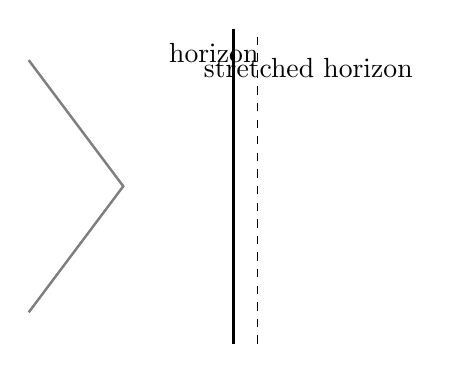
\begin{tikzpicture}[scale=1.0]
\draw[gray,thick] (-2.0,1.6) -- (-0.8,0) -- (-2.0,-1.6);
\draw[gray,thick] (-2.0,-1.6) -- (-0.8,0) -- (-2.0,1.6);
\draw[thick] (0.6,-2.0) -- (0.6,2.0);
\draw[dashed] (0.9,-2.0) -- (0.9,2.0);
\node at (0.35,1.7) {horizon};
\node at (1.55,1.5) {stretched horizon};
\end{tikzpicture}
\caption{A cleaned reconstruction of the lecture's alternate picture: the horizon drawn as a vertical boundary, together with a nearby stretched horizon one Planck length away.}
\end{figure}

The conceptual gain is important. The horizon is not merely a geometric boundary. It is the place where the high-frequency quantum fluctuations become real thermal phenomena for the outside observer. This is exactly the perspective Susskind wants to carry over to cosmic horizons.

\section{De Sitter Geometry From Expanding Coordinates To Causal Diagrams}

With the black-hole analogy in place, the lecture turns to de Sitter space. The starting point is the exponentially expanding flat slicing,
\begin{equation}
ds^2=-dt^2+e^{2Ht}\,d\mathbf{x}^2,
\qquad
d\mathbf{x}^2=dx^2+dy^2+dz^2.
\end{equation}
A fixed coordinate separation \(\Delta x\) therefore corresponds to a physical separation
\begin{equation}
\Delta x_{\text{phys}}(t)=e^{Ht}\,\Delta x.
\end{equation}
This is why de Sitter space is drawn as an exponentially expanding geometry.

Susskind then wants a coordinate system in which future infinity fits on the board and light rays run at \(45^\circ\). In the transcript the sign bookkeeping is corrected in real time, so it is best to present the standard conformal-time form that captures the point of the lecture:
\begin{equation}
\eta=-\frac{1}{H}e^{-Ht},
\qquad
t\to +\infty \Longrightarrow \eta\to 0^-.
\end{equation}
In terms of \(\eta\), the metric becomes
\begin{equation}
ds^2=\frac{1}{H^2\eta^2}\left(-d\eta^2+d\mathbf{x}^2\right).
\end{equation}
Now the conformal factor is irrelevant for null motion, so radial light rays satisfy
\begin{equation}
ds^2=0
\qquad\Longrightarrow\qquad
d\eta=\pm dx.
\end{equation}
This is the practical reason for the coordinate change. It turns causal structure into simple Euclidean geometry on the board.

\begin{figure}
\centering
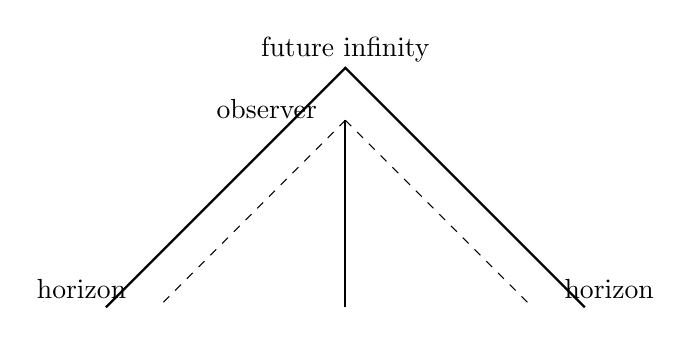
\begin{tikzpicture}[scale=0.95]
\draw[thick] (-3.2,0) -- (0,3.2) -- (3.2,0);
\draw[thick] (0,0) -- (0,2.5);
\draw[dashed] (0,2.5) -- (-2.5,0);
\draw[dashed] (0,2.5) -- (2.5,0);
\draw (-0.25,2.65) node[left] {observer};
\draw (0,3.45) node {future infinity};
\draw (-2.8,0.25) node[left] {horizon};
\draw (2.8,0.25) node[right] {horizon};
\end{tikzpicture}
\caption{Transcript-led conformal reconstruction of one de Sitter observer and the backward light cone that defines the accessible region.}
\end{figure}

This diagram captures the next major conceptual step. For a single eternal observer, the physically relevant universe is not the whole de Sitter spacetime. It is the backward light cone of that observer. Other observers have different accessible regions, with partial overlap, but the lecture deliberately narrows to one observer at a time.

\section{The Observer's Horizon And The Static Patch}

At this point the de Sitter picture still looks time dependent. The backward light cone narrows as one moves upward in the conformal diagram, and it is tempting to think that the observer's horizon is shrinking. Susskind then inserts a short calculation to show that this impression is wrong.

\paragraph{A worked horizon-distance calculation.}
Take two points on a constant-\(\eta\) slice, one at the observer and one on the horizon. Since there is no time separation, only the spatial part of the metric contributes. On such a slice,
\begin{equation}
D^2=\frac{(\Delta x)^2}{H^2\eta^2}.
\end{equation}
But in the conformal diagram the horizon line is at \(45^\circ\), so the horizontal coordinate distance to the horizon is equal to the vertical conformal-time coordinate:
\begin{equation}
\Delta x=|\eta|.
\end{equation}
Substituting gives
\begin{align}
D^2&=\frac{\eta^2}{H^2\eta^2}=\frac{1}{H^2},\\
D_{\text{hor}}&=\frac{1}{H}.
\end{align}
Thus the physical distance to the horizon is constant. This is the calculation that motivates the next coordinate system.

If the horizon size is time independent for a single observer, one expects an observer-adapted coordinate patch in which the metric itself is static. Susskind does not derive the transformation in detail. He simply writes the answer, correcting a sign slip as he goes:
\begin{equation}
ds^2=-(1-H^2r^2)\,dt^2+\frac{dr^2}{1-H^2r^2}+r^2\,d\Omega_2^2.
\end{equation}
This is the static patch, also called the causal patch.

\begin{figure}
\centering

\includegraphics[width=0.72\textwidth]{lecture_09_figure_04.png}
\caption{Static-patch metric and de Sitter horizon radius on the lecture board.}
\end{figure}

Susskind immediately compares this with the Schwarzschild metric. The comparison is structural rather than derivational. In Schwarzschild one has the familiar factor
\begin{equation}
1-\frac{2MG}{r},
\end{equation}
while in the de Sitter static patch the corresponding factor is
\begin{equation}
1-H^2r^2.
\end{equation}
In both cases the horizon is where this factor vanishes. Thus
\begin{equation}
1-H^2r^2=0
\qquad\Longrightarrow\qquad
r=\frac{1}{H},
\end{equation}
in agreement with the conformal-diagram calculation.

The lecture's point is not that the two spacetimes are globally the same. They are not. The point is that near the horizon the redshift structure is so similar that the same thermodynamic logic applies. The black-hole horizon is observed from the outside; the de Sitter horizon is observed from the inside. But the near-horizon mathematics is closely related.

\section{Vacuum Energy, Redshift, And Late-Time de Sitter Physics}

The static patch makes the de Sitter redshift story concrete. We are at \(r=0\), the horizon is at \(r=1/H\), and photons emitted near the horizon are severely redshifted on their way inward. Locally, near the horizon, the same high-energy horizon physics is present as in the black-hole case. At the center, however, the observed de Sitter temperature is tiny.

Susskind estimates the present de Sitter horizon scale as
\begin{equation}
\frac{1}{H}\sim 20\times 10^9\ \text{light years}.
\end{equation}
That scale explains why the radiation is so cold for us. The redshift is enormous, and the corresponding wavelengths are absurdly large, of order billions of light years. This is why the de Sitter temperature seen at the center has nothing to do with the microwave background and is far too small for ordinary laboratory detection.

He dramatizes the operational distinction with the same thought experiment used for black holes. Alice sits at the center and keeps an ordinary thermometer there. It reads an extremely low temperature. But if she sends a thermometer outward, on a very long line, toward the horizon and later reads the returned signal, the temperature read near the horizon is high. The geometry is the same, but the viewpoint is reversed: for de Sitter one performs the experiment from the inside.

The lecture then returns to a student's question: in the black-hole case one can talk about a gravitational well. What plays the analogous role in de Sitter space? Susskind answers with a deliberately heuristic Newtonian exercise.

\begin{figure}
\centering

\includegraphics[width=0.60\textwidth]{lecture_09_figure_05.png}
\caption{Poisson equation and radial potential form on the lecture board.}
\end{figure}

He introduces a Newtonian potential \(\phi\), defined so that its gradient gives the force on a test mass, and writes a Poisson equation schematically as
\begin{equation}
\nabla^2\phi=\rho.
\end{equation}
For a radially symmetric distribution he then simplifies it, at lecture level, to
\begin{equation}
\frac{d^2\phi}{dr^2}=\rho.
\end{equation}

\begin{remark}
In the lecture Susskind explicitly leaves the overall sign convention unresolved, and the radial equation is only a heuristic simplification. The purpose of the argument is to identify the quadratic dependence on \(r\), not to present an exact spherically symmetric Poisson analysis.
\end{remark}

Now insert a constant source, representing vacuum energy or cosmological constant, with magnitude set by \(H^2\) up to conventions:
\begin{equation}
\rho_{\text{vac}}\propto H^2.
\end{equation}
A constant on the right-hand side means that \(\phi\) should be quadratic in \(r\). Up to signs and factors of order unity, the lecture arrives at
\begin{equation}
\phi(r)\propto -H^2r^2.
\end{equation}
Then
\begin{equation}
F_r=-\frac{d\phi}{dr}\propto +H^2r,
\end{equation}
so the force is repulsive and grows linearly with distance. This is the Newtonian shadow of exponential expansion.

\begin{figure}
\centering

\includegraphics[width=0.72\textwidth]{lecture_09_figure_06.png}
\caption{Newtonian-style potential sketch for de Sitter repulsion on the lecture board.}
\end{figure}

\begin{figure}
\centering
\begin{tikzpicture}[scale=0.95]
\draw[->] (-0.3,0) -- (5.4,0) node[right] {$r$};
\draw[->] (0,-2.5) -- (0,2.6) node[above] {$\phi$};
\draw[thick] (0,2.0) parabola bend (2.6,1.1) (5.0,-2.1);
\draw[dashed] (4.1,-2.5) -- (4.1,2.5);
\node at (4.1,2.8) {$r=1/H$};
\end{tikzpicture}
\caption{Clean reconstruction of the lecture's upside-down de Sitter potential.}
\end{figure}

This picture also lets Susskind fold ordinary gravity back in. If one adds the usual attractive \( -GM/r \) contribution to the upside-down quadratic term, the result is a combined potential with a local maximum. Inside that maximum, attraction wins; outside it, cosmological repulsion wins. That is the lecture's qualitative explanation of why Andromeda can still fall toward us while sufficiently distant galaxies accelerate away.

The far-future interpretation now becomes stark. A few hundred billion years from now, almost everything not gravitationally bound will have disappeared beyond the horizon. The observer's patch will be nearly empty except for extremely feeble horizon radiation. Future astronomers may inherit a world in which the microwave background has redshifted away, distant galaxies are gone, and the direct observational evidence for cosmology has almost vanished.

\section{Thermal Fate: Recurrences, Rare Fluctuations, And Boltzmann Brains}

Once the observer's patch has been made into a static thermal system, Susskind moves naturally into statistical mechanics. De Sitter space is now treated as a cavity with a finite entropy and a very low temperature at the center. At lecture level, the entropy is simply the horizon area in Planck units:
\begin{equation}
S_{\text{dS}}\sim \frac{A_{\text{hor}}}{\ell_P^2}.
\end{equation}
What matters here is not the exact numerical factor, but finiteness. A finite-entropy thermal system fluctuates.

Susskind first recalls the standard thermal lesson from a box of gas. Equilibrium looks dull only on short time scales. On sufficiently long time scales, rare fluctuations occur. The probability of a large fluctuation is exponentially small in the entropy cost, and the corresponding waiting time is exponentially large:
\begin{equation}
P(\text{rare fluctuation})\sim e^{-S_{\text{dS}}},
\qquad
t_{\text{rec}}\sim e^{S_{\text{dS}}}.
\end{equation}
For de Sitter space this becomes unimaginably large. In the lecture it is described schematically as a recurrence time of order \(e^{10^{120}}\) in whatever units one likes.

More modest fluctuations are cheaper. If an object \(X\) has entropy \(S_X\), then one expects
\begin{equation}
P_X\sim e^{-S_X}.
\end{equation}
This is how the lecture builds its sequence of ever cheaper fluctuations. A fluctuation that recreates an entire Big Bang is fantastically expensive. A fluctuation producing a solar system is cheaper. One producing only an Earth is cheaper still. Cheapest of all, if all one wants is an observer, might be the nucleation of a single functioning brain.

That is the path to the Boltzmann-brain problem. If a cosmology predicts that the overwhelmingly dominant observers are brains created by thermal fluctuations rather than ordinary observers with a long cosmological history, then something has gone badly wrong with the cosmological picture. The point is not comic. It is a sharp diagnostic of whether the statistical mechanics of the universe has been posed correctly.

\section{Eternal Inflation, The Measure Problem, And A String-Theory Coda}

The final large extension of the lecture is from one de Sitter patch to an eternally inflating spacetime. Susskind sketches the idea of bubble nucleation: a de Sitter region can be unstable to the appearance of bubbles in which the cosmological constant is smaller. Each bubble expands, and many bubbles form at later times. The population of bubbles grows exponentially.

\begin{figure}
\centering
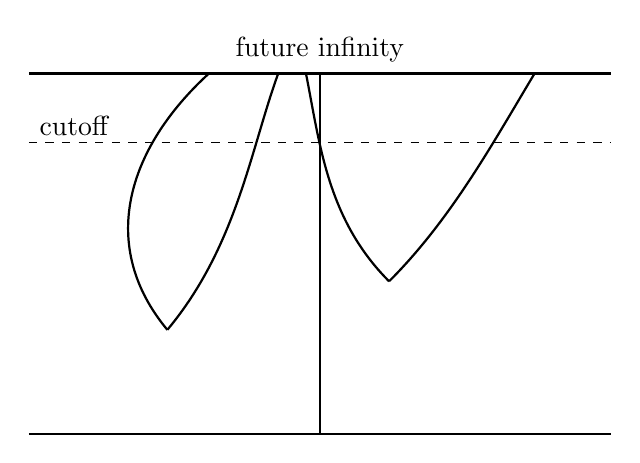
\begin{tikzpicture}[scale=0.88]
\draw[thick] (-4.2,0) -- (4.2,0);
\draw[thick] (0,0) -- (0,5.2);
\draw[thick] (-4.2,5.2) -- (4.2,5.2);
\draw[thick] (-2.2,1.5) .. controls (-3.2,2.7) and (-2.8,4.1) .. (-1.6,5.2);
\draw[thick] (-2.2,1.5) .. controls (-1.2,2.7) and (-1.0,4.1) .. (-0.6,5.2);
\draw[thick] (1.0,2.2) .. controls (0.1,3.1) and (0.0,4.2) .. (-0.2,5.2);
\draw[thick] (1.0,2.2) .. controls (1.9,3.1) and (2.5,4.2) .. (3.1,5.2);
\draw[dashed] (-4.2,4.2) -- (4.2,4.2);
\node at (0,5.55) {future infinity};
\node at (-3.55,4.45) {cutoff};
\end{tikzpicture}
\caption{Transcript-led schematic of bubble nucleation in an inflating background. The dashed line represents a cutoff, and the measure problem is that bubble counts depend sensitively on how such a cutoff is imposed.}
\end{figure}

The measure problem enters because counting in an exponentially growing population is treacherous. Susskind gives several examples, but the simplest mathematical model is a doubling population. If one counts backward from the end, the newest generation makes up half of all people who ever lived, the newest two generations make up three-quarters, and the newest three generations make up seven-eighths. In the idealized doubling model,
\begin{equation}
f_{\text{last }n\text{ generations}}=1-2^{-n}.
\end{equation}
Thus the assumption that we are ``typical'' in such a population pushes us toward the edge.

This is the logic behind the lecture's examples of finite resources, Escher's devils near the boundary of a drawing, and bubble universes near a chosen cutoff surface. The central problem is not merely that there are many observers. It is that the answer to probability questions becomes extremely sensitive to how one cuts off the exponentially growing set before counting it. That is what Susskind calls the measure problem.

The lecture ends with a short string-theory coda. The function of that coda is modest. Susskind emphasizes that the mathematically precise part of string theory is highly constrained, internally consistent, and includes gravity and quantum mechanics, but it is supersymmetric in a way the observed world is not. In that sense, the fully controlled version of string theory is not the real world. The real hope is that it sits inside a larger structure, one not yet understood with comparable mathematical precision. This is an ending about scope and rigor, not a new derivational theme.

\section{Summary}

The lecture begins with a student's question about hot horizons and never really leaves it. Black-hole redshift separates the hot local near-horizon region from the much cooler Hawking temperature seen far away. The same logic, carried into de Sitter space, leads to the conformal diagram, the constant horizon distance \(1/H\), and the static patch metric for one observer. A heuristic Newtonian analysis then models vacuum energy by a repulsive quadratic potential, clarifying both de Sitter redshift and accelerated expansion. Once the observer's world has become a finite-entropy thermal patch, heat death, recurrences, Boltzmann brains, eternal inflation, and the measure problem appear not as disconnected curiosities, but as the statistical afterlife of horizon thermodynamics.